%==============================================================================
% introduction.tex
%==============================================================================

\chapter{Introduction}
\label{chap:introduction}

Intervals \cite{Matsakis2009a} are a new, higher-level primitive for
multi-threaded programming allowing programmers to directly construct
the program schedule. They are under active development at ETH Zürich
as part of the PhD research of Nicholas D. Matsakis
\cite{Matsakis2010}.

The intervals implementation in Java uses a work-stealing scheduler
where a worker running out of work tries to ``steal'' work from
others. The scope of this thesis is to improve the performance of the
intervals scheduler.


\section{Intervals}
\label{sec:intro-intervals}

Traditional primitives for synchronizing multi-threaded programs, such
as semaphores and barriers, are low-level and dangerous to use. They
require careful attention to implementation details to achieve good
performance, and are prone to errors, especially deadlocks and race
conditions.\footnote{Section \ref{sec:intro-intervals} summarizes the
  introduction to intervals written by \textcite{Matsakis2010a}.}

Intervals are a higher-level alternative that make parallel
programming more secure while maintaining the flexibility and
efficiency of threads. When using intervals, programmers create
lightweight tasks and order them using \emph{happens before} relations
\cite{Lamport1978}. Programmers need not specify when tasks should
block or acquire a lock. Instead they define when a task should
execute in relation to other tasks, and what locks it should hold
during execution. It is the duty of the runtime system to make this
schedule pass.

The intervals API supports arbitrary \emph{happens before} relations
making the model very flexible. Intervals can be used to emulate
existing thread primitives \cite{Matsakis2009a}, but they can also be
used to create program schedules for which no standard thread
primitives exist, such as peer-to-peer synchronization.

Intervals can be extended to support both dynamic and static checks
such as data race protection \cite{Matsakis2010b} and checking for
deadlocks \cite{Matsakis2009}. An error in one task prevents other,
dependent tasks from executing \cite{Matsakis2010a}.

\subsection{Model}
\label{sec:intro-intervals-model}

Intervals are first-class objects in the programming language which
stand for the slice of program time used to execute a parallel task.
They are structured in a tree with the root representing the entire
program execution.

The conceptual model for intervals consists of points in time ordered
by a \emph{happens before} relation. In the model, an interval
\lstinline!i! consists of a pair of points -- \lstinline!i.start! and
\lstinline!i.end! -- called the start and end point. They the start
and end of the interval's execution. Programmers may define arbitrary
ordering constraints by adding \emph{happens before} edges in between
the start or end points of different intervals. An edge
\lstinline!p1 $\rightarrow$ p2! indicates that the point
\lstinline!p1! must occur before the point \lstinline!p2!. It also
guarantees that any memory writes which \emph{happen before}
\lstinline!p1! must be visible to \lstinline!p2!. This is in line with
the Java Memory Model \cite{Manson2005}, and the semantics of volatile
fields and synchronized sections.

\begin{figure}[htb]
  \centering
  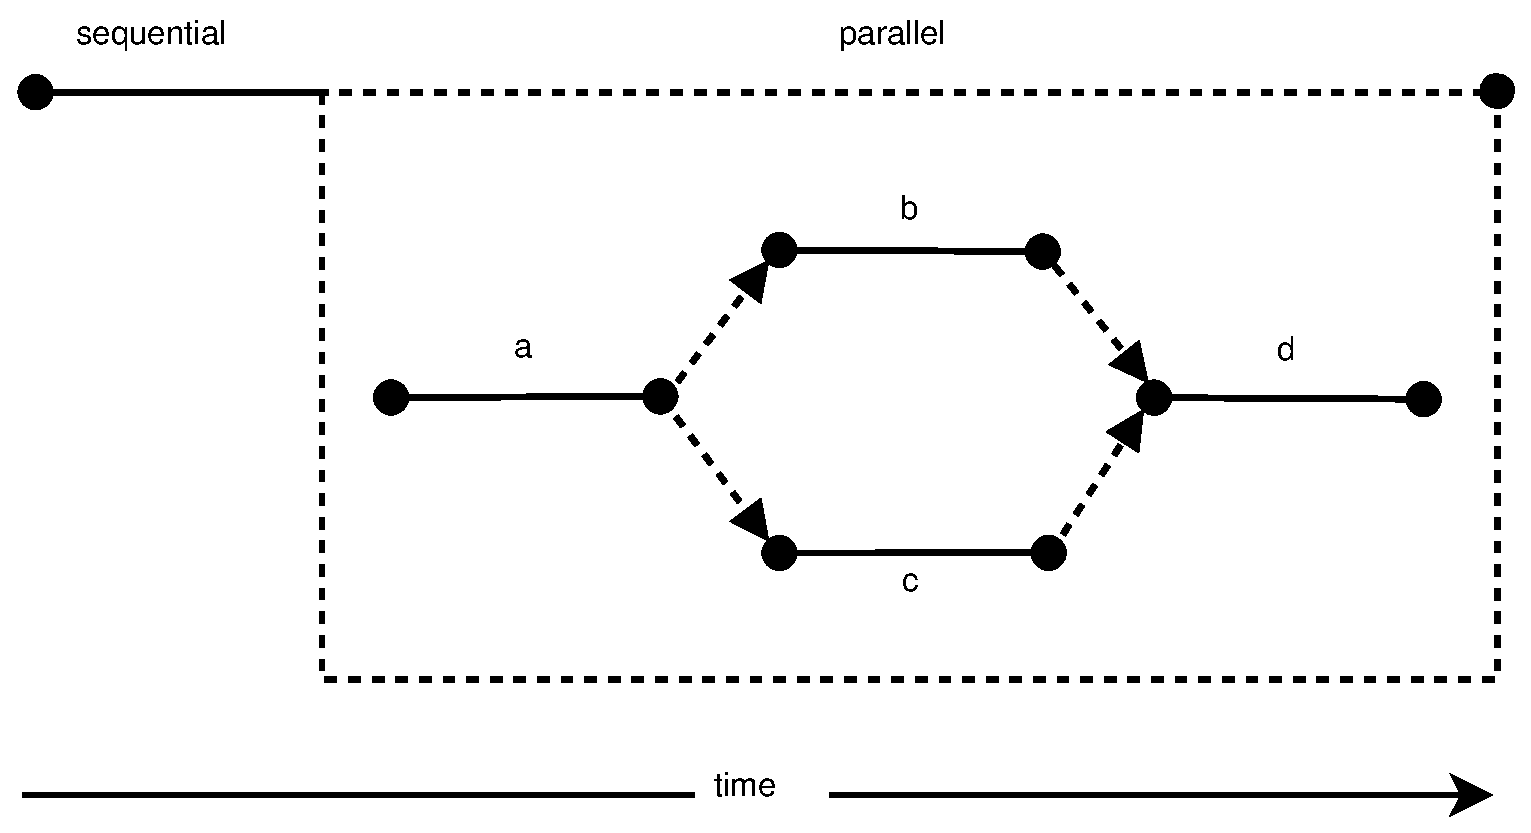
\includegraphics[width=0.96\textwidth]{introduction/interval-graph}
  \caption[Example interval graph]{Example interval graph: Showing an
    interval and its subintervals \lstinline!a!, \lstinline!b!,
    \lstinline!c! and \lstinline!d!.}
  \label{fig:introduction-interval-graph}
\end{figure}

An interval can have one or more locks. The intervals runtime
automatically acquires those locks before the interval's start point
occurs. When the task is completed and the end point of the interval
has occurred, the acquired locks are released again.

When an interval executes, it begins by calling the sequential
\lstinline!run()! method. The \lstinline!run()! method can either
execute the task directly or create a number of subintervals to solve
the task in parallel.

The interval model can be depicted as a graph, as shown in Figure
\ref{fig:introduction-interval-graph}. The graph contains a single
interval with four subintervals, \lstinline!a!, \lstinline!b!,
\lstinline!c! and \lstinline!d!. The start and end points of each
interval are drawn as opaque circles. The subintervals of an interval
are enclosed in a dashed box which is left out for leaf intervals.

The dashed edges connecting different points indicate \emph{happens
  before} relations added by the programmer. For example, the end of
\lstinline!a! \emph{happens before} the start of \lstinline!b! and
\lstinline!c! and the ends of \lstinline!b! and \lstinline!c! both
\emph{happen before} the start of \lstinline!d!.

\subsection{Java API}
\label{sec:intro-intervals-java-api}

To create an interval programmers have to subclass the abstract class
\lstinline!Interval! (Listing \ref{lst:introduction-interval-class})
and redefine the \lstinline!run()! method. Besides the abstract
\lstinline!run()! method, \lstinline!Interval! features final fields
to access the start and end point as well as the parent interval.

\begin{lstlisting}[
  style=Float, 
  caption={[\lstinline{Interval} class] \lstinline{Interval}: Base class for all intervals},
  label=lst:introduction-interval-class
]
public abstract class Interval {
  public final Interval parent;
  public final Point start;
  public final Point end;

  protected abstract void run();
}
\end{lstlisting}

Listing \ref{lst:introduction-interval-graph} shows the code used to
construct the graph shown in Figure
\ref{fig:introduction-interval-graph}.

\begin{lstlisting}[
  style=FloatNumbers, 
  caption={[Intervals Java API example] Code to construct the sample interval graph shown in Figure \ref{fig:introduction-interval-graph}},
  label=lst:introduction-interval-graph
]
public class ExampleInterval extends Interval {
  public ExampleInterval(Dependency dep, String name) {
    super(dep, name);
  }
  
  protected void run() {
    // Task
  }
  
  public static void main(String[] args) {
    Intervals.inline(new VoidInlineTask() { //*\label{lst:introduction-interval-graph-inline-start}
      public void run(Interval start) {
        Interval a = new ExampleInterval(start, "a"); //*\label{lst:introduction-interval-graph-new-start}
        Interval b = new ExampleInterval(start, "b");
        Interval c = new ExampleInterval(start, "c");
        Interval d = new ExampleInterval(start, "d"); //*\label{lst:introduction-interval-graph-new-end}
        
        Intervals.addHb(a, b); //*\label{lst:introduction-interval-graph-add-hb}
        Intervals.addHb(a, c);
        Intervals.addHb(b, d);
        Intervals.addHb(c, d);
        Intervals.schedule(); //*\label{lst:introduction-interval-graph-schedule}
      }
    }); //*\label{lst:introduction-interval-graph-inline-end}
  }
}
\end{lstlisting}

\subsubsection{Creating Intervals}
\label{sec:intro-intervals-creating-intervals}

To start program execution, the programmer has to create a new child
of the root interval, for example by using an inline interval. Inline
intervals execute a task during the current interval and do not return
until the task has completed.

Lines \ref{lst:introduction-interval-graph-inline-start} --
\ref{lst:introduction-interval-graph-inline-end} create an inline interval by
providing an anonymous task class redefining its \lstinline!run()!
method. The interval has four subintervals, \lstinline!a!,
\lstinline!b!, \lstinline!c! and \lstinline!d!. They are created on
Lines \ref{lst:introduction-interval-graph-new-start} --
\ref{lst:introduction-interval-graph-new-end} and are normal, non-blocking
intervals.

\subsubsection{Scheduling Intervals}
\label{sec:intro-intervals-scheduling-intervals}

Newly constructed intervals become eligible for execution once the
\lstinline!schedule()! method is invoked, as shown on Line
\ref{lst:introduction-interval-graph-schedule} in Listing
\ref{lst:introduction-interval-graph}. This gives the user the
opportunity to construct any required dependencies or perform other
initialization. For example, adding the edge
\lstinline!a $\rightarrow$ b! on Line
\ref{lst:introduction-interval-graph-add-hb} would be unsafe if
\lstinline!b! could begin immediately, as it would be possible that
\lstinline!b.start! had already occurred before the call to
\lstinline!addHb()! could add the new dependency.

Explicit calls to \lstinline!schedule()! are unusual as the runtime
automatically invokes \lstinline!schedule()! when the
\lstinline!run()! method of an interval returns.


\section{Work-Stealing Scheduler}
\label{sec:intro-work-stealing-scheduler}

The implementation of intervals for Java makes use of a work-stealing
scheduler similar to those found in Cilk \cite{Blumofe1995,
  Frigo1998}, Java 7 \cite{Lea2000, Lea2000a, Lea2004, Lea2006}, Intel
Threading Building Blocks \cite{Reinders2007, Contreras2008}, or
Microsoft Task Parallel Library \cite{Leijen2009} but extended to
support locks and happens before edges.

A work-stealing scheduler employs a fixed number of threads called
workers. Each worker has a local double-ended queue, or deque, to
maintain its own pool of ready tasks from which it obtains work. When
a worker finds that its pool is empty, it becomes a thief and steals a
task from the pool of a victim worker chosen at random.

To obtain work, a worker takes the ready task from the tail of its
deque and executes it. If the task terminates, the worker goes back to
the tail of its deque to take off another task upon which it can
work. When assigning a new task to a worker, the worker puts the newly
ready task onto the tail of its deque. Thus, so long as a worker's
deque is not empty, the worker manipulates its deque in a LIFO
(stack-like) manner.

When a worker tries to obtain work by taking a task off the tail of
its deque and it finds that it is empty, then the worker becomes a
thief. It picks a victim worker at random and attempts to obtain work
by removing the task at the head of the victim worker's deque. If the
victim worker's deque is empty, then the thief picks another victim
worker and tries again until it finds a victim whose deque it
non-empty. At which point the thief continues to work on the stolen
task as described above. Since steals take place at the head of the
victim's deque, stealing operates in a FIFO manner.

Accessing the run queues at different ends offers several advantages
\cite{Frigo1998}:

\begin{itemize}
\item It reduces contention by having owner and thieves working on
  opposite sides of the deque.
\item Recursive divide-and-conquer algorithms generate ``large'' tasks
  early. Thus, the older stolen task is likely to further provide more
  work to the stealing worker.
\item Stealing a task also migrates its future workload, which helps
  to increase locality.
\end{itemize}

The assignment of tasks to workers for execution is done in a provably
efficient manner \cite{Blumofe1995, Blumofe1999}.


\section{Overview}
\label{sec:intro-overview}

In \autoref{part:locality} of the thesis we implement and analyze an
advanced scheduler for intervals. It is designed for locality-aware
scheduling using locality hints provided by the programmer. Instead of
using work-stealing workers, our scheduler groups workers into
\emph{Work-Stealing Places}.  Each work-stealing place has a fixed
number of workers and a local deque to maintain ready tasks. The
workers of a place share its local deque from which they obtain
work. When a worker finds that its place's pool is empty, it becomes a
thief and steals a task from the pool of a victim place chosen at
random. When an interval with affinity for a place is ready for
scheduling, it gets added to the place it has affinity for.

In the non-blocking work-stealing algorithm, the deques are
implemented with non-blocking synchronization \cite{Arora1998}. The
current deque implementation of intervals however uses mutual
exclusion when trying to steal. As a separate effort, we design and
explore alternative non-blocking queue implementations with the aim to
improve work-stealing performance (\autoref{part:queues}).


%%% Local Variables: 
%%% mode: latex
%%% TeX-master: "thesis"
%%% End: 
